\chapter{Result}
\paragraph*{}
This chapter details the result of our project through images of our demonstration achieving our objectives.

\begin{figure}[H]
    \centering
    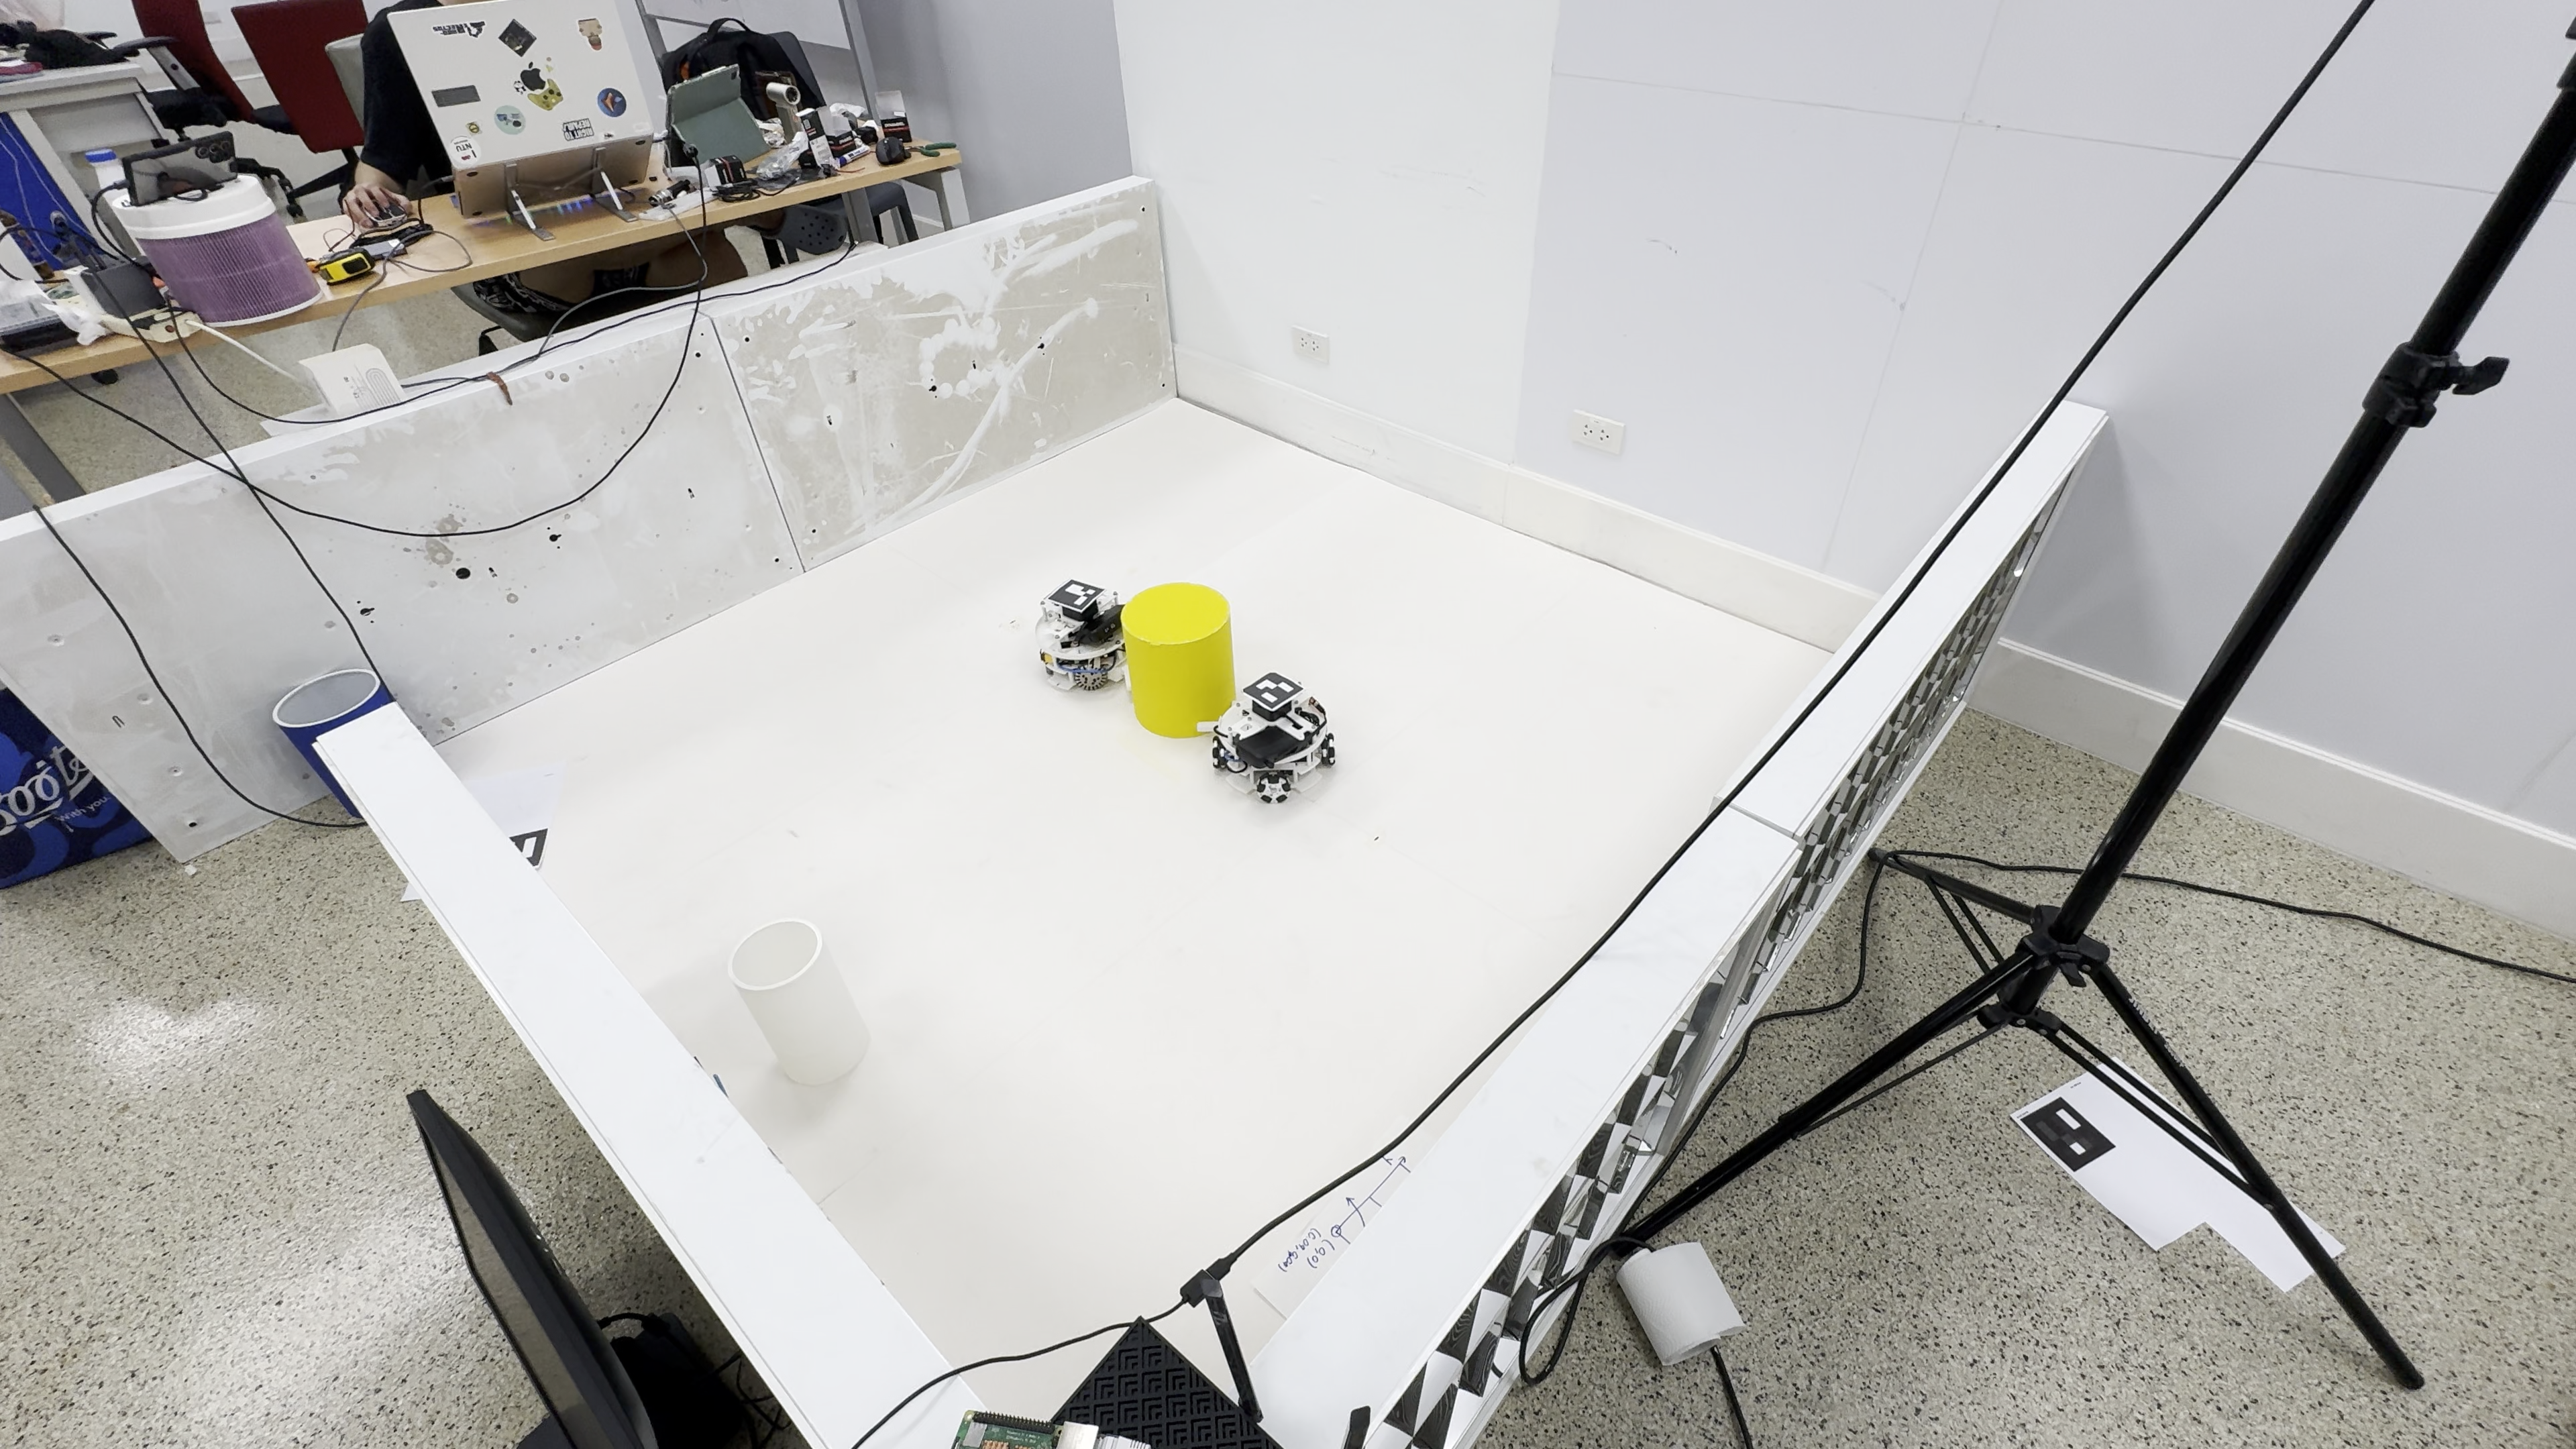
\includegraphics[width=1\linewidth]{assets/images/result-demo/RealDemo-0007.png}
    \caption{Robot moving towards object}
    \label{fig:detail-result}
\end{figure}

\paragraph*{}
The image above shows the robots successfully moving towards the object in a synchronized manner.

\begin{figure}[H]
    \centering
    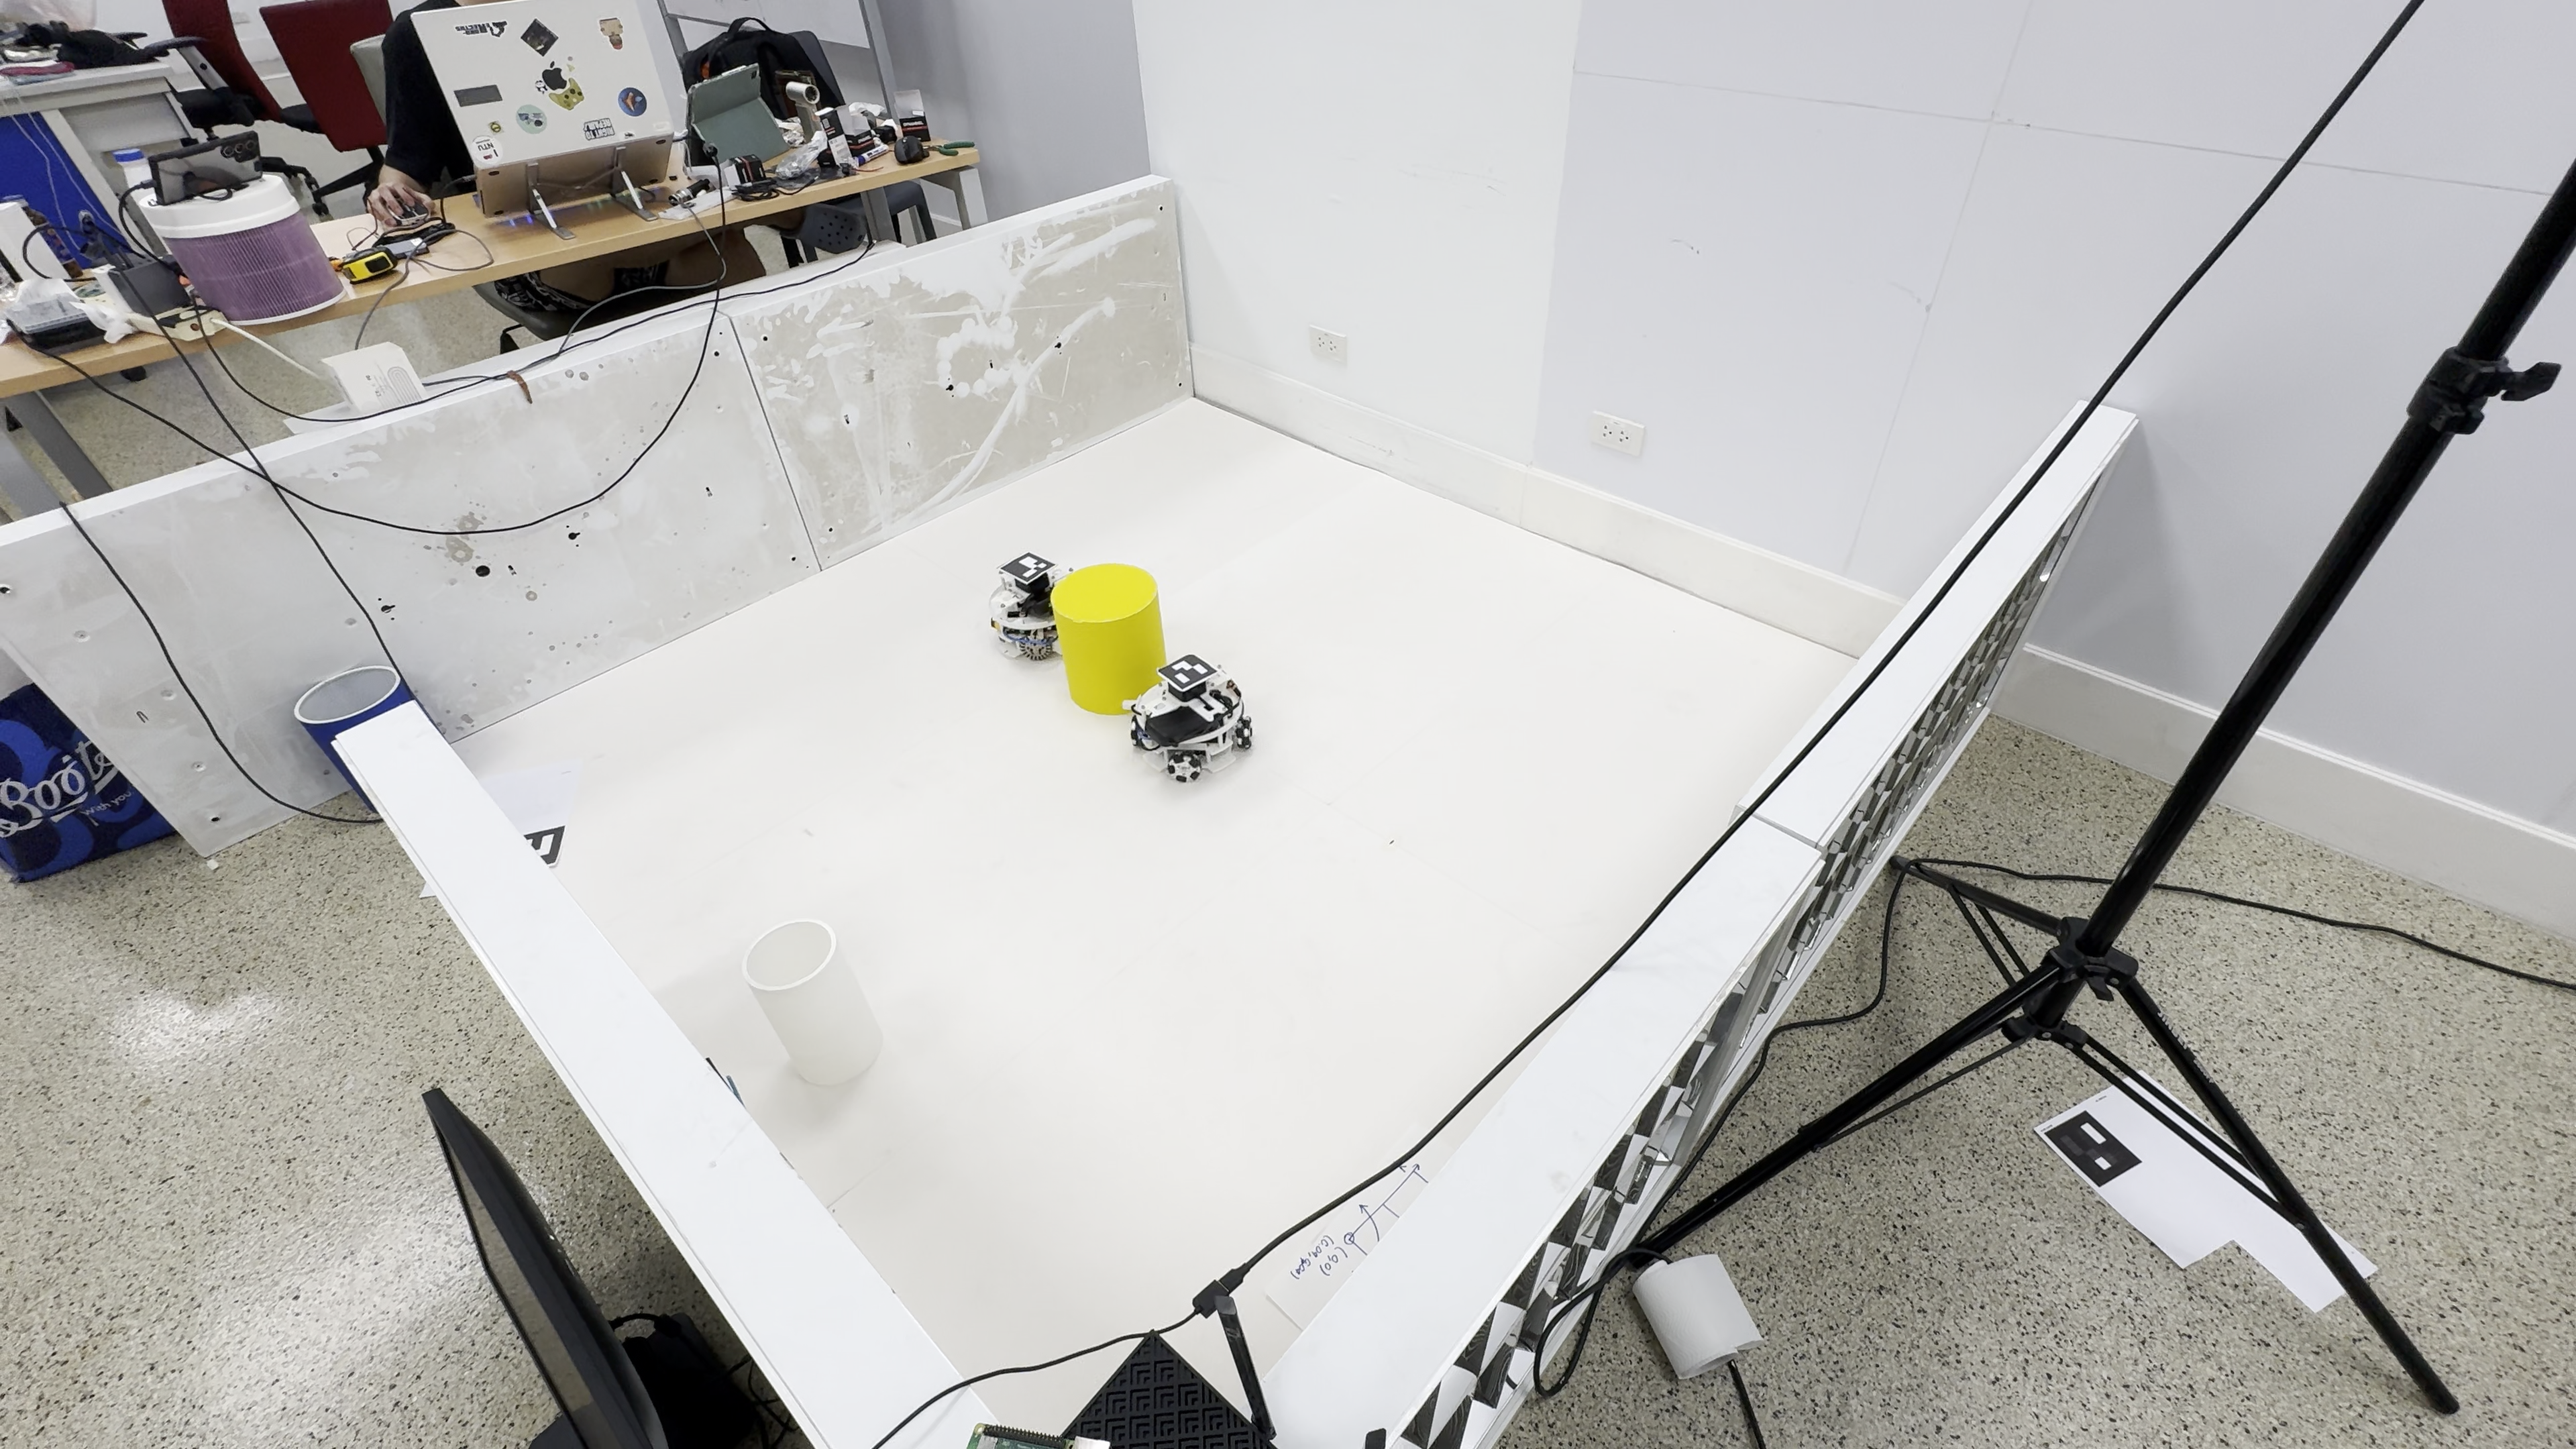
\includegraphics[width=1\linewidth]{assets/images/result-demo/RealDemo-0008.png}
    \caption{Robots grip and transport object}
    \label{fig:detail-result}
\end{figure}

\paragraph*{}
The image shows how the robots grip the object at the correct position. The robots then transports the object collectively in the global y direction

\begin{figure}[H]
    \centering
    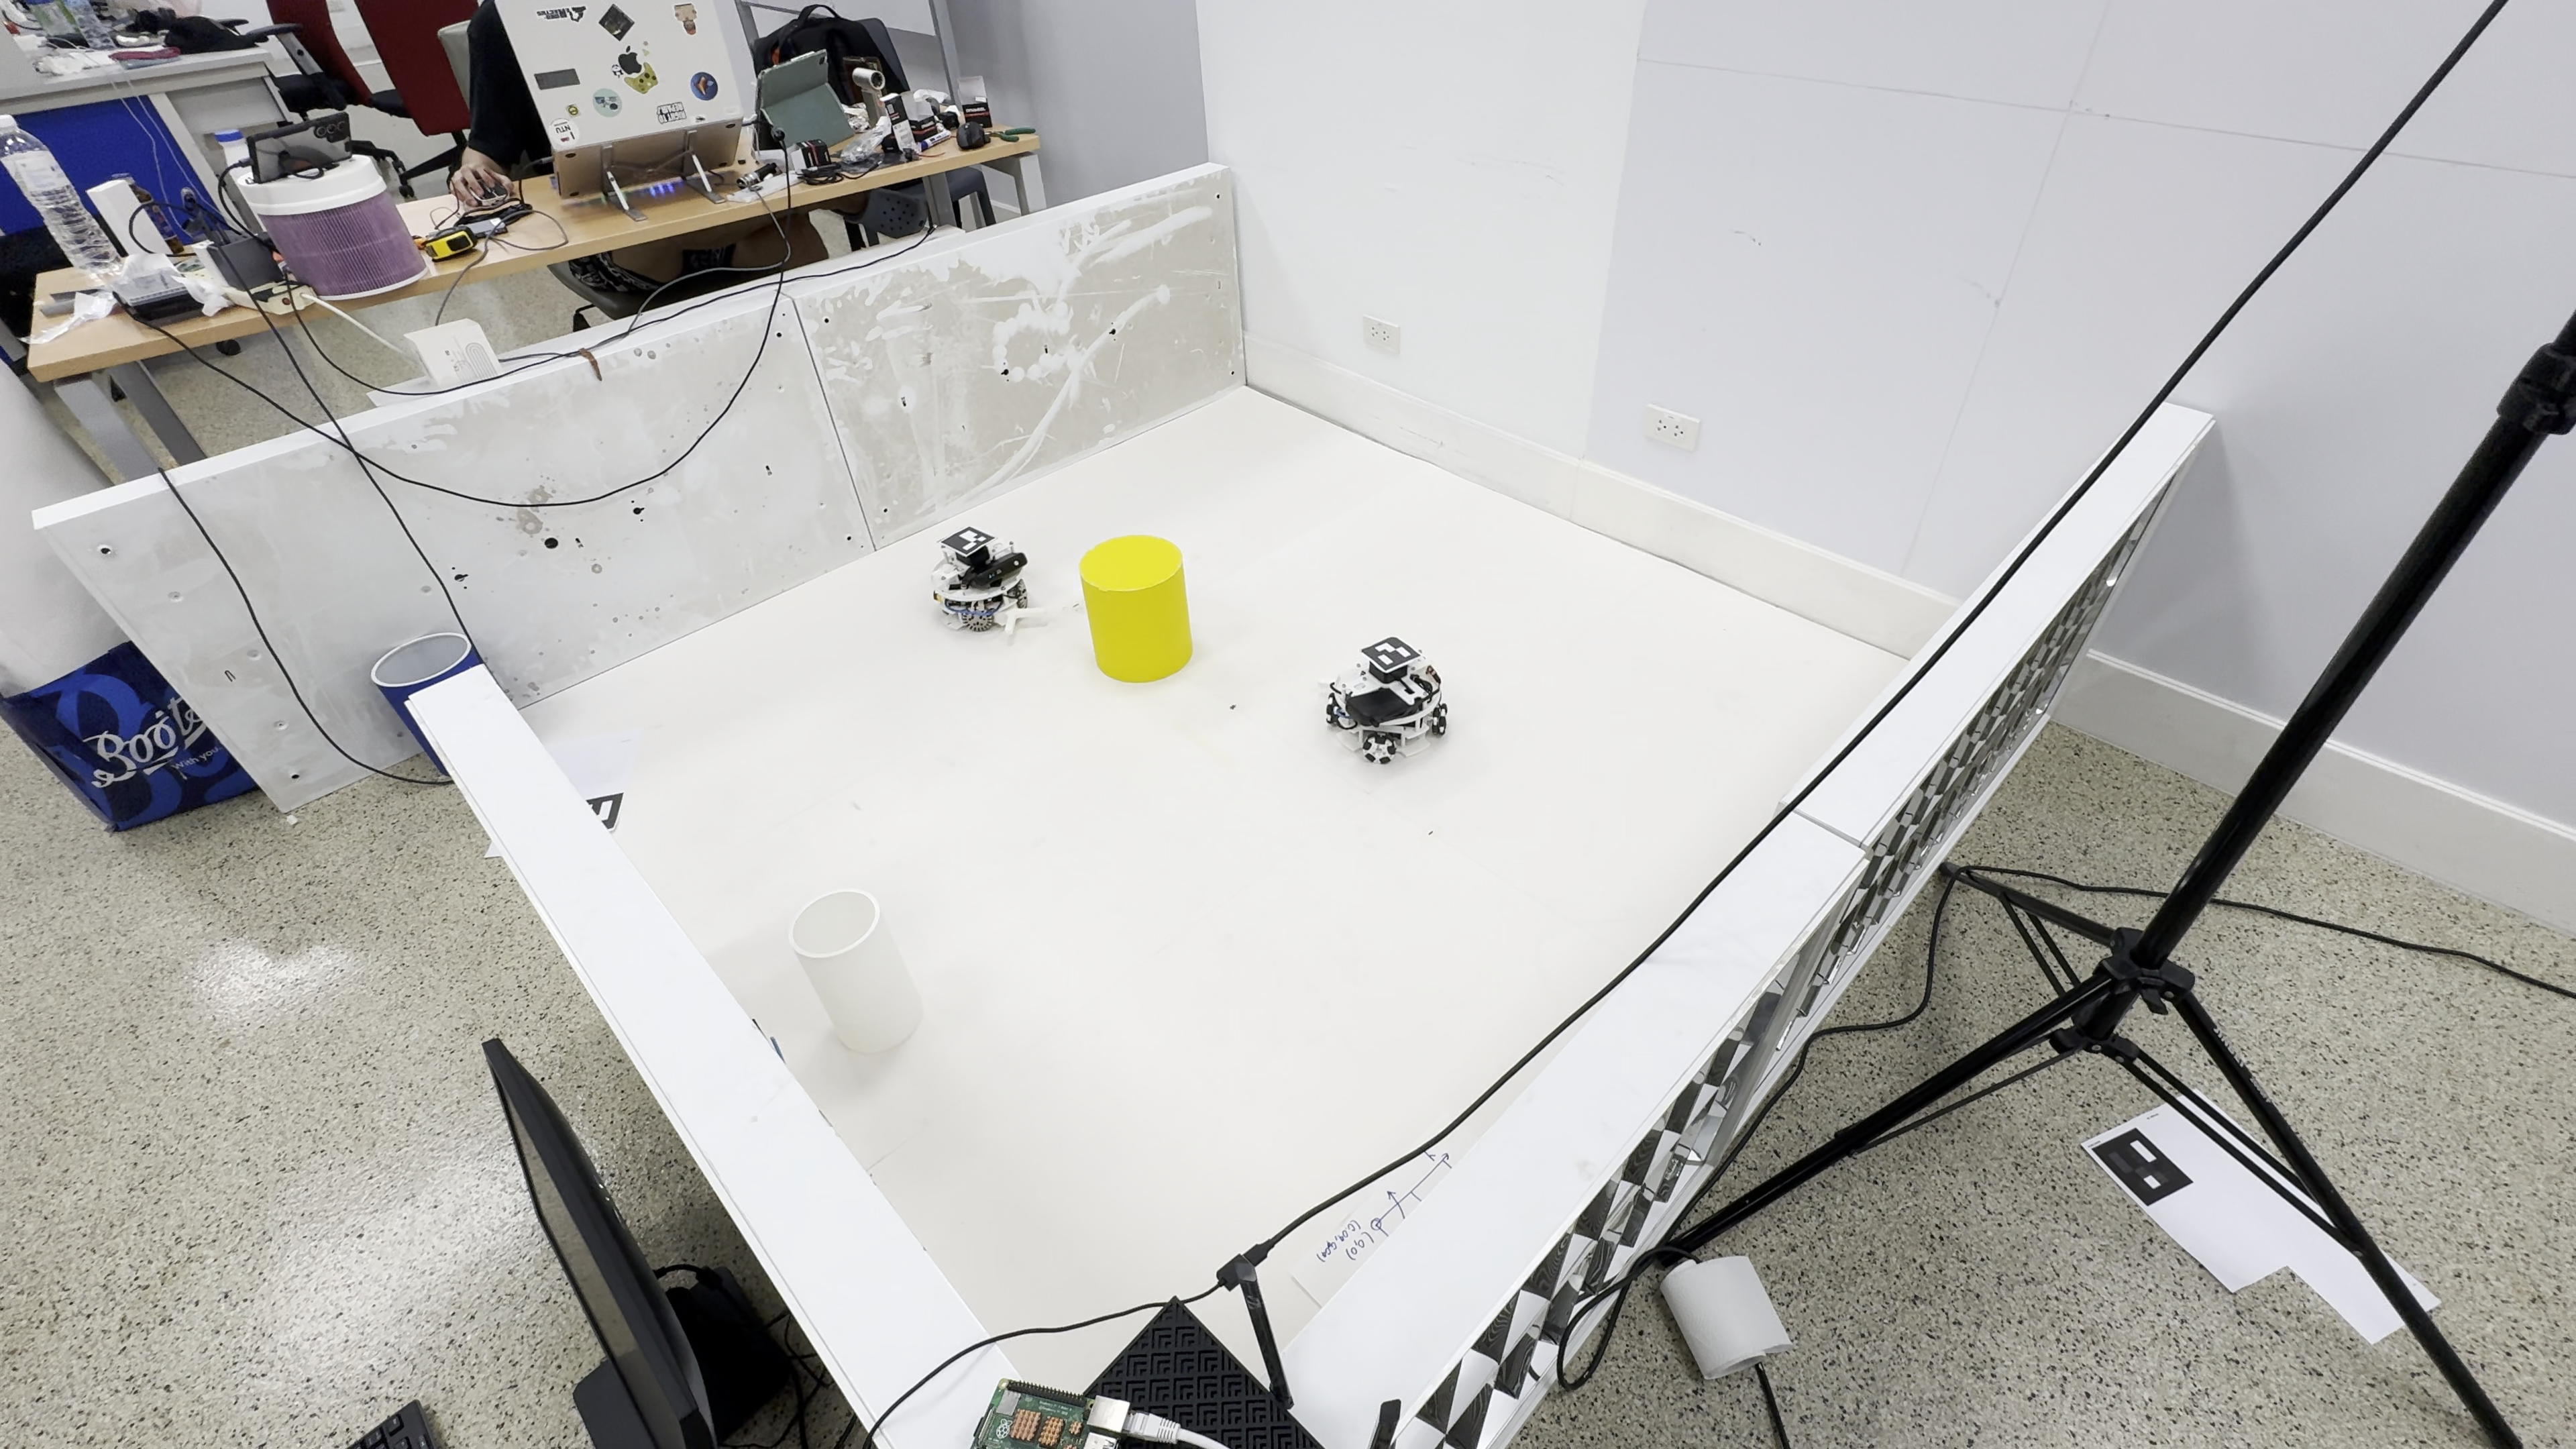
\includegraphics[width=1\linewidth]{assets/images/result-demo/RealDemo-0009.png}
    \caption{Robots return to Home position}
    \label{fig:detail-result}
\end{figure}

\paragraph*{}
After transporting the object the robots then move towards their home positions

\begin{figure}[H]
    \centering
    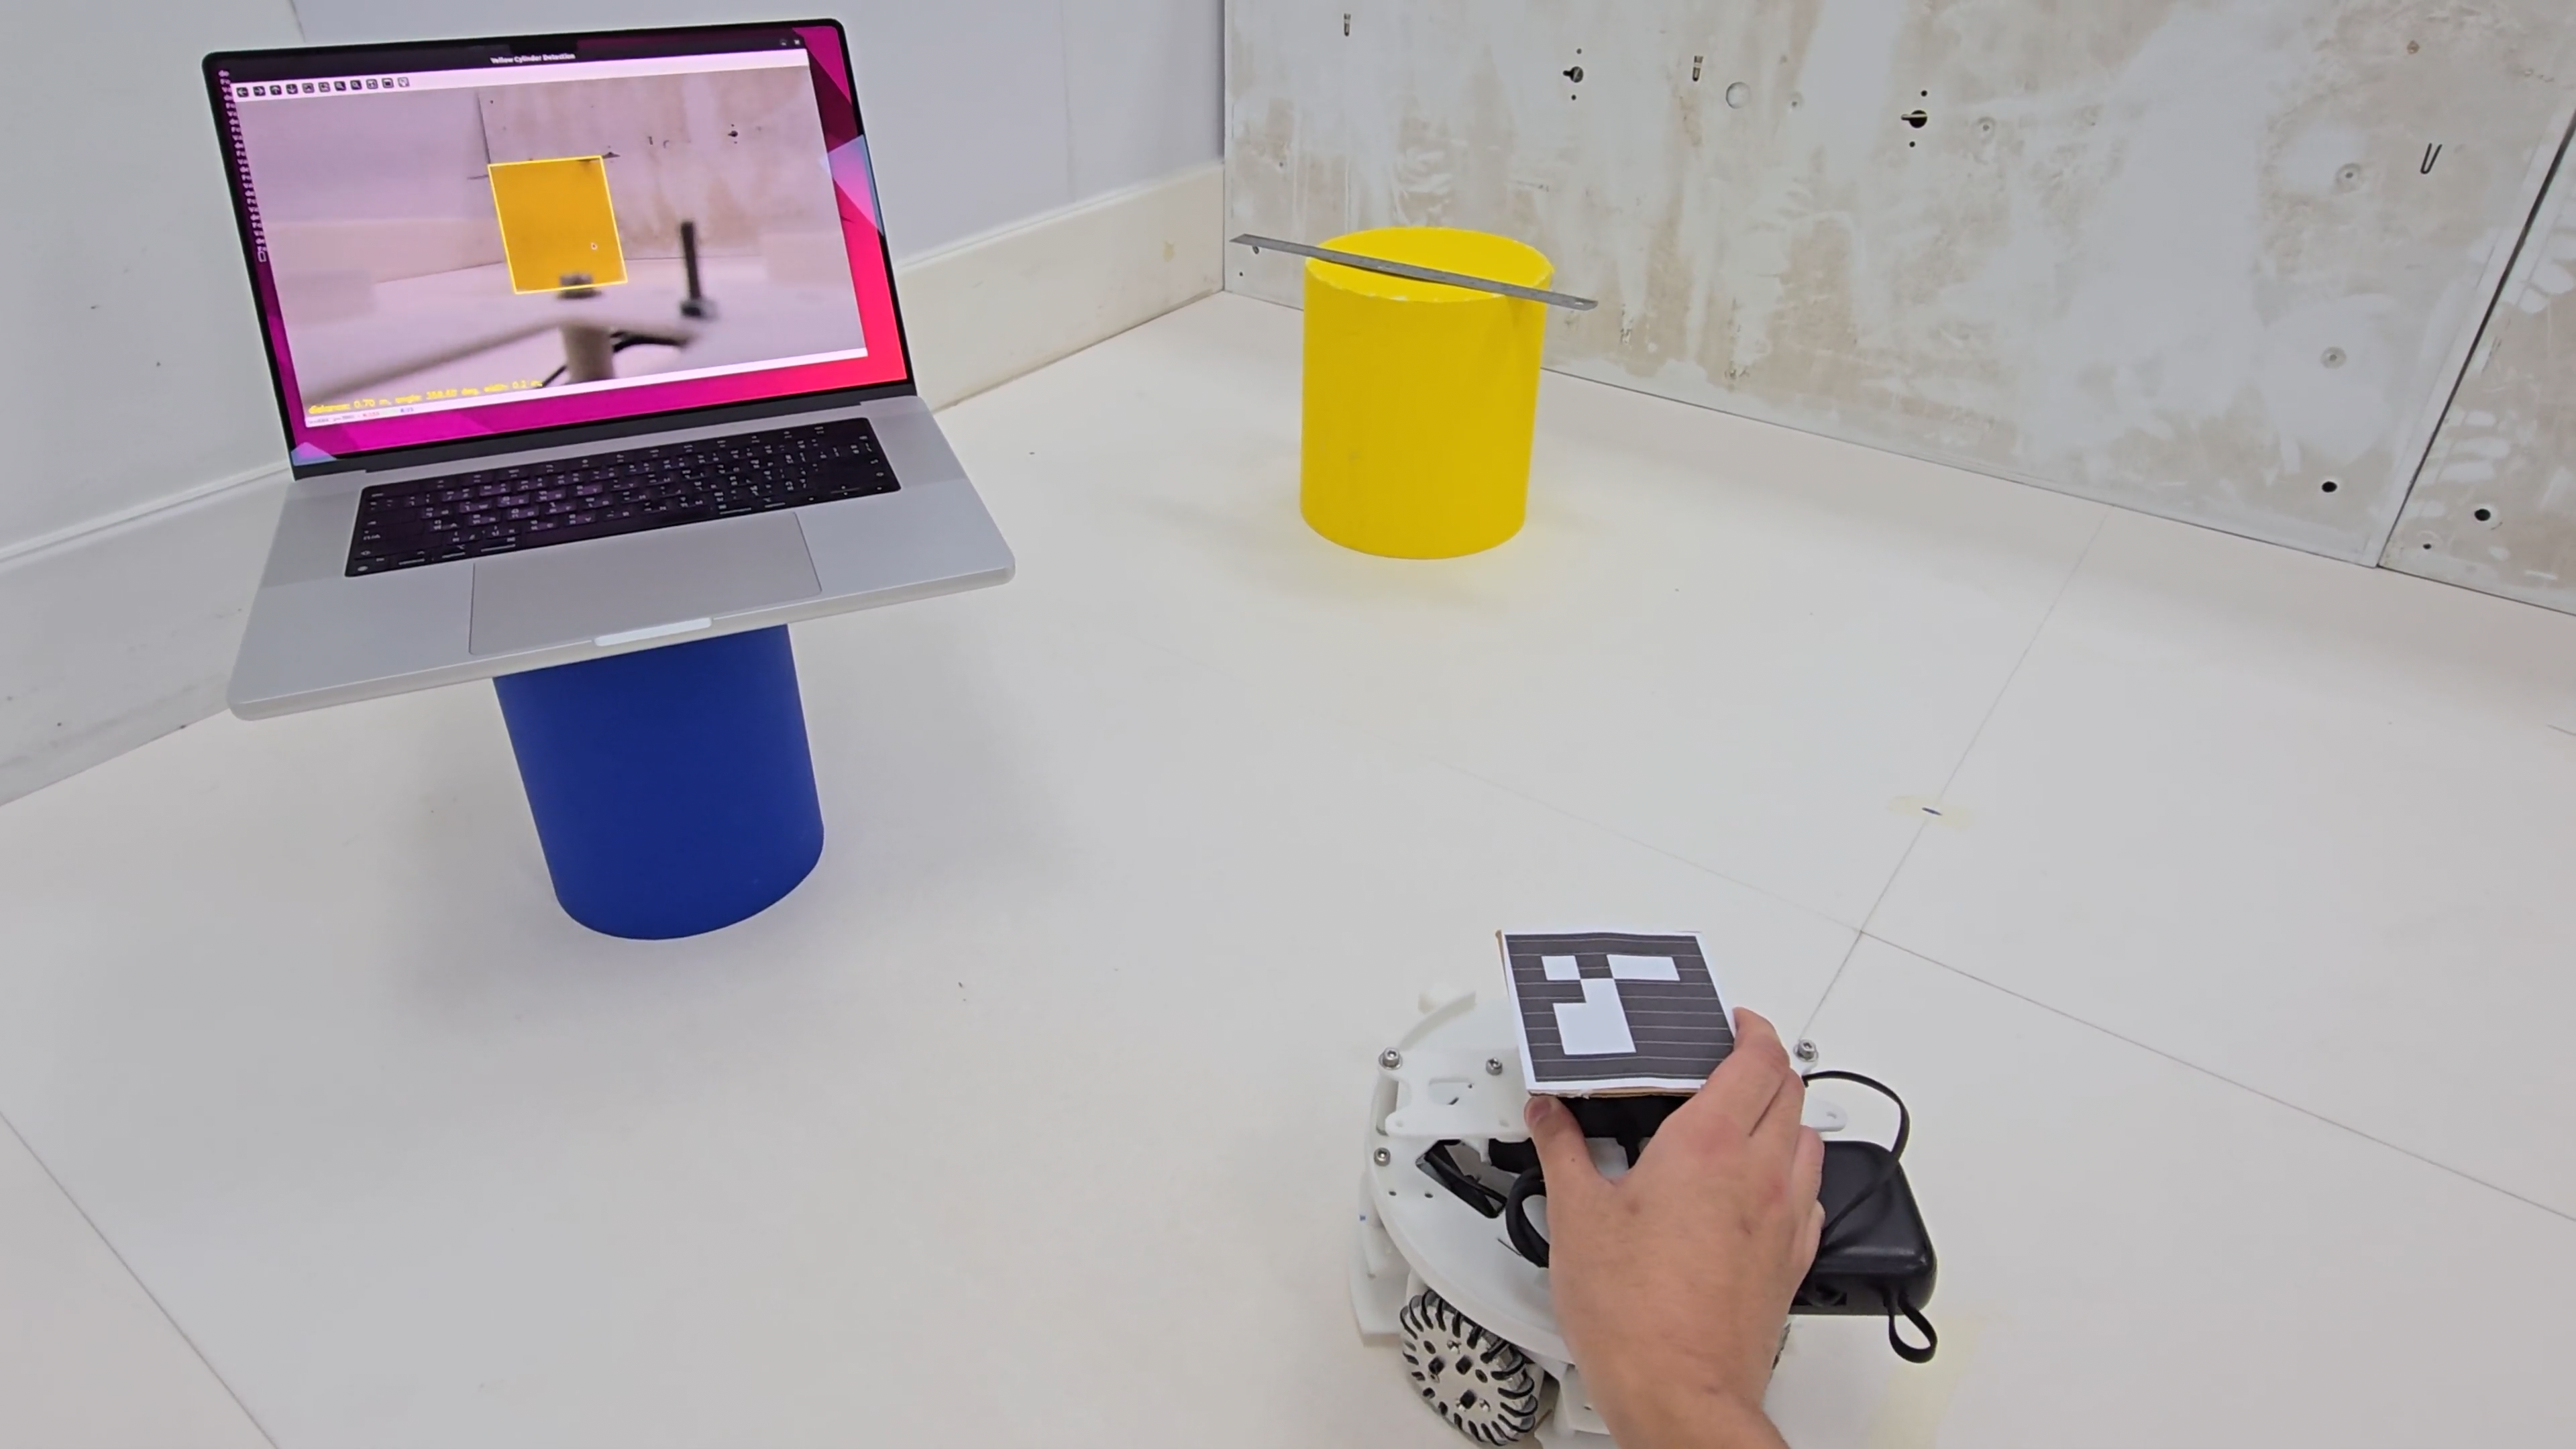
\includegraphics[width=1\linewidth]{assets/images/result-demo/AccurateCV 114-5-25-01:26-abr7500-0001.png}
    \caption{Robot detecting object}
    \label{fig:detail-result}
\end{figure}

\paragraph*{}
The above image shows how the robot detects an object by creating the box around it

\begin{figure}[H]
    \centering
    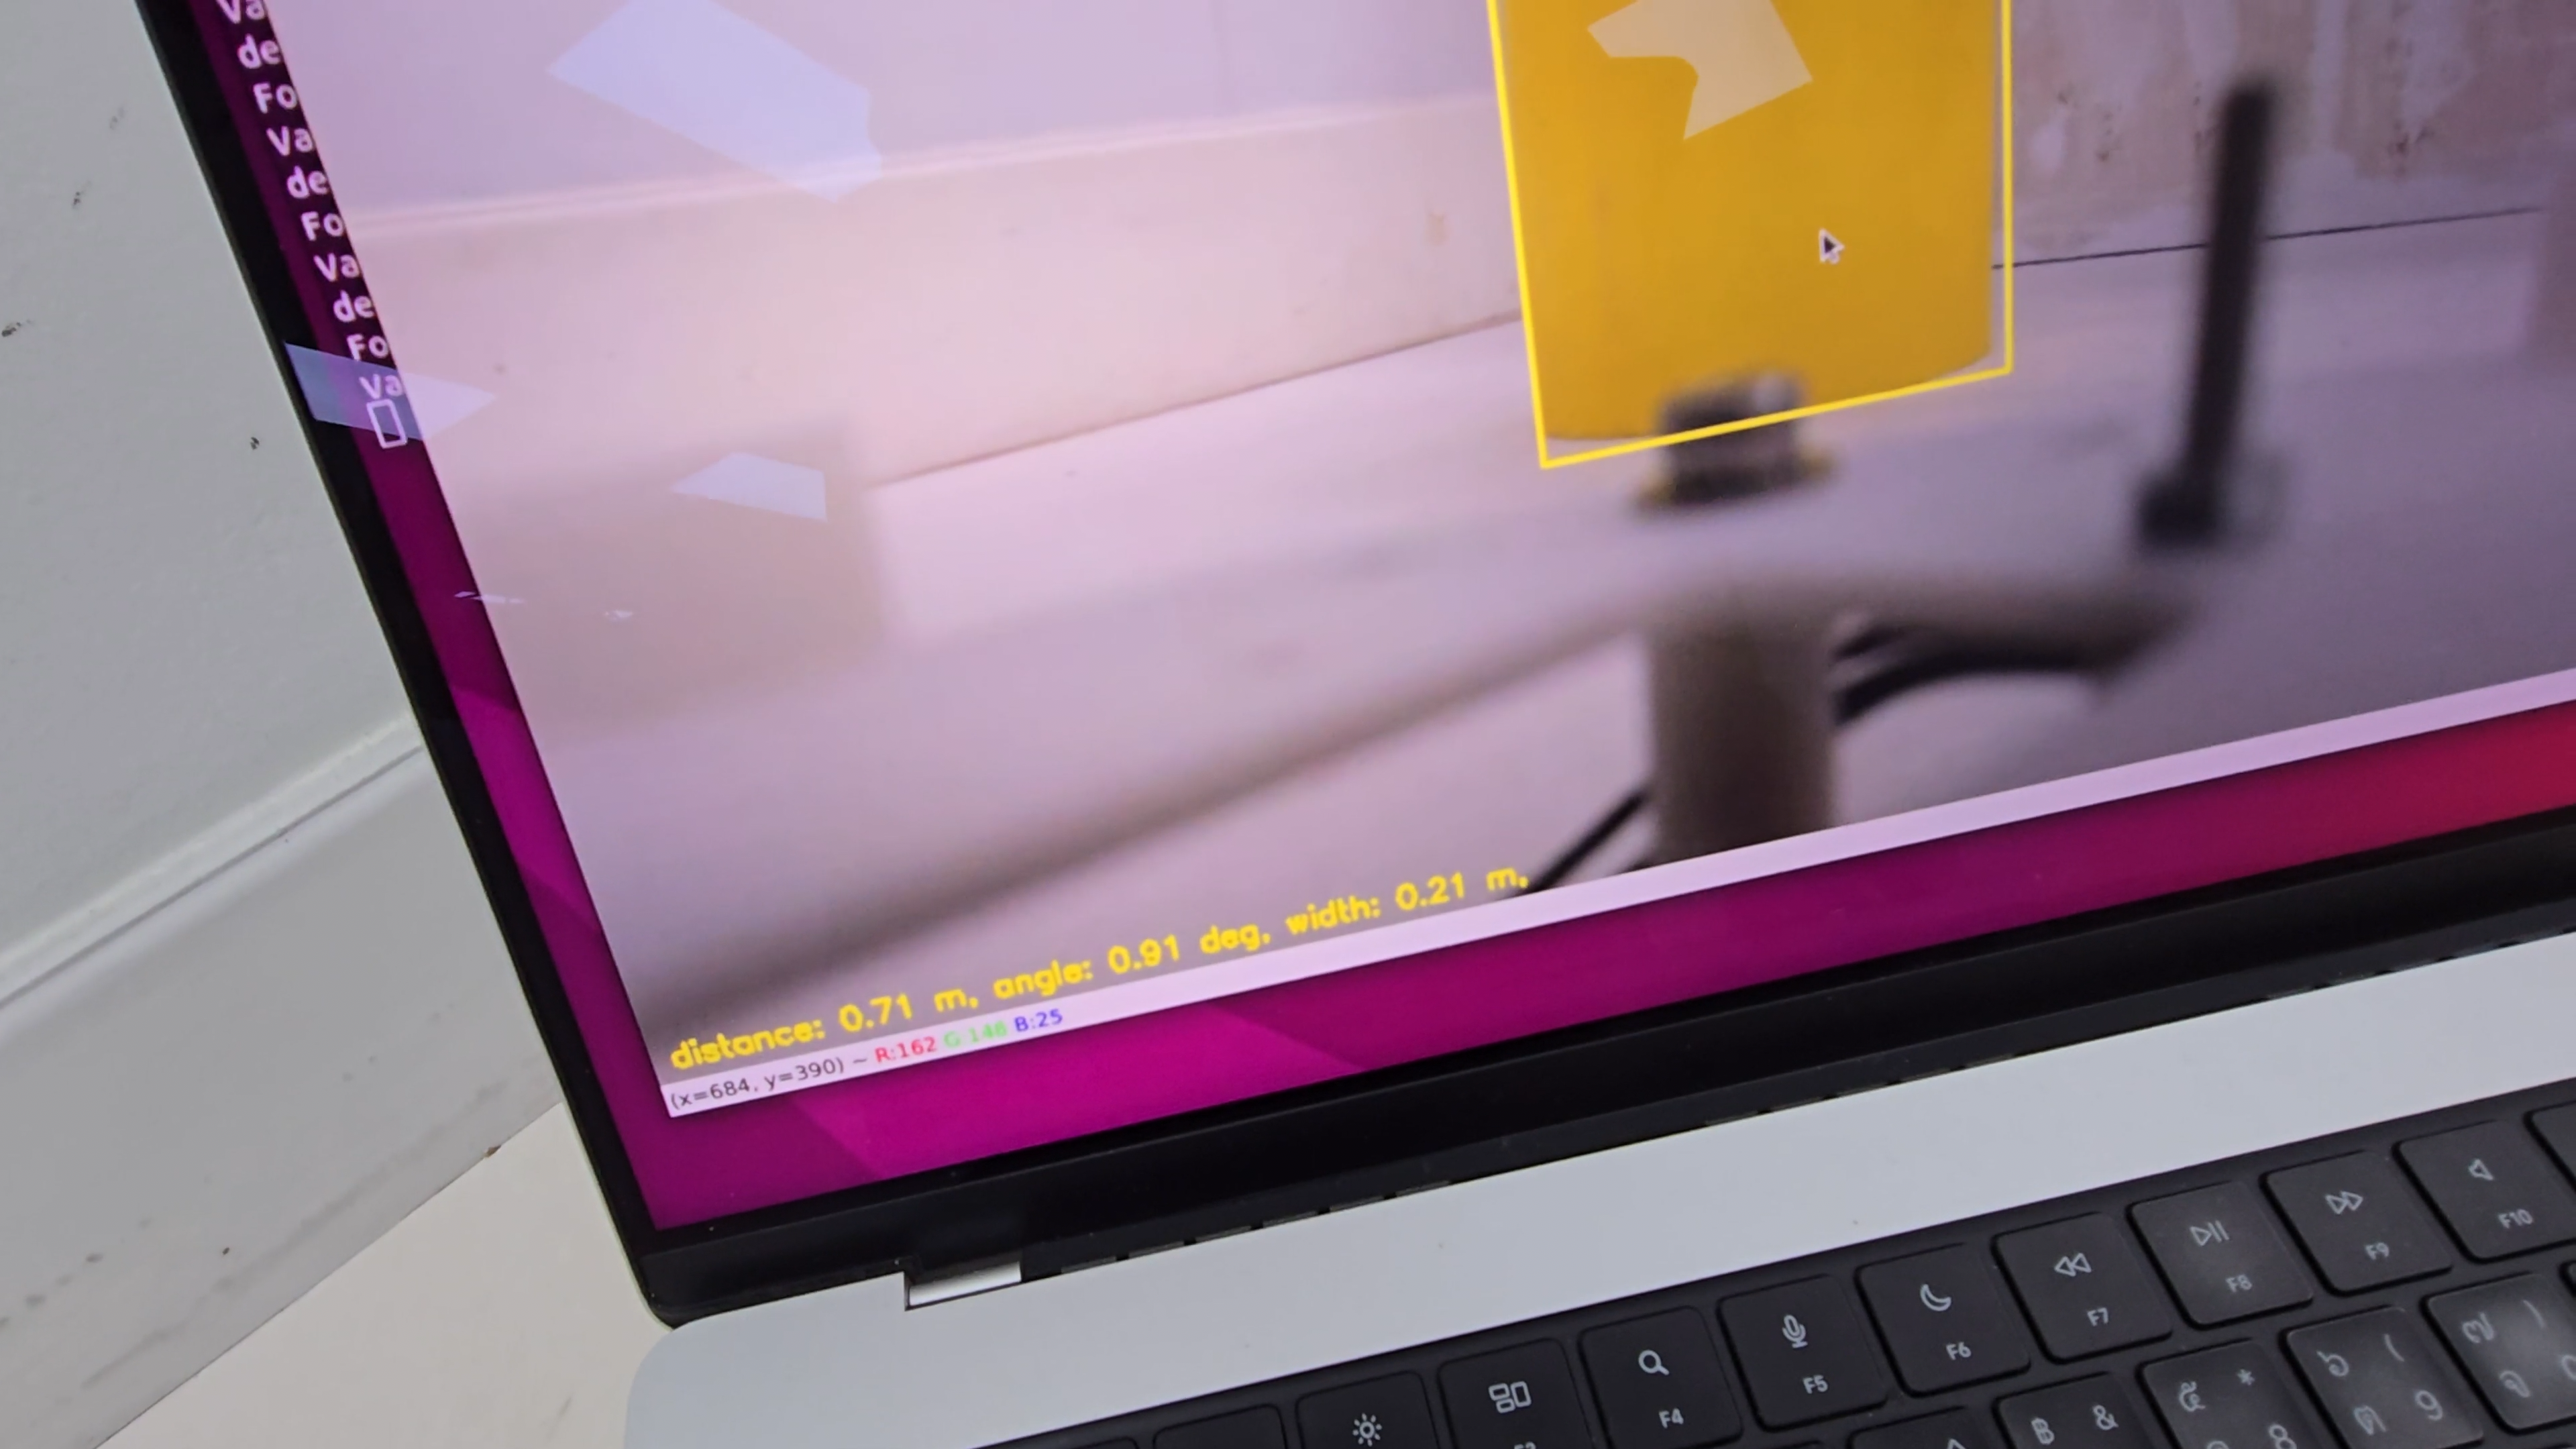
\includegraphics[width=1\linewidth]{assets/images/result-demo/AccurateCV 114-5-25-01:26-abr7500-0002.png}
    \caption{Measurements of the object}
    \label{fig:detail-result}
\end{figure}

\paragraph*{}
The object detection module then processes the measurements necessary. The distance between the object and the robot, the angle between the object and the robot, and the width of the object.

\begin{figure}[H]
    \centering
    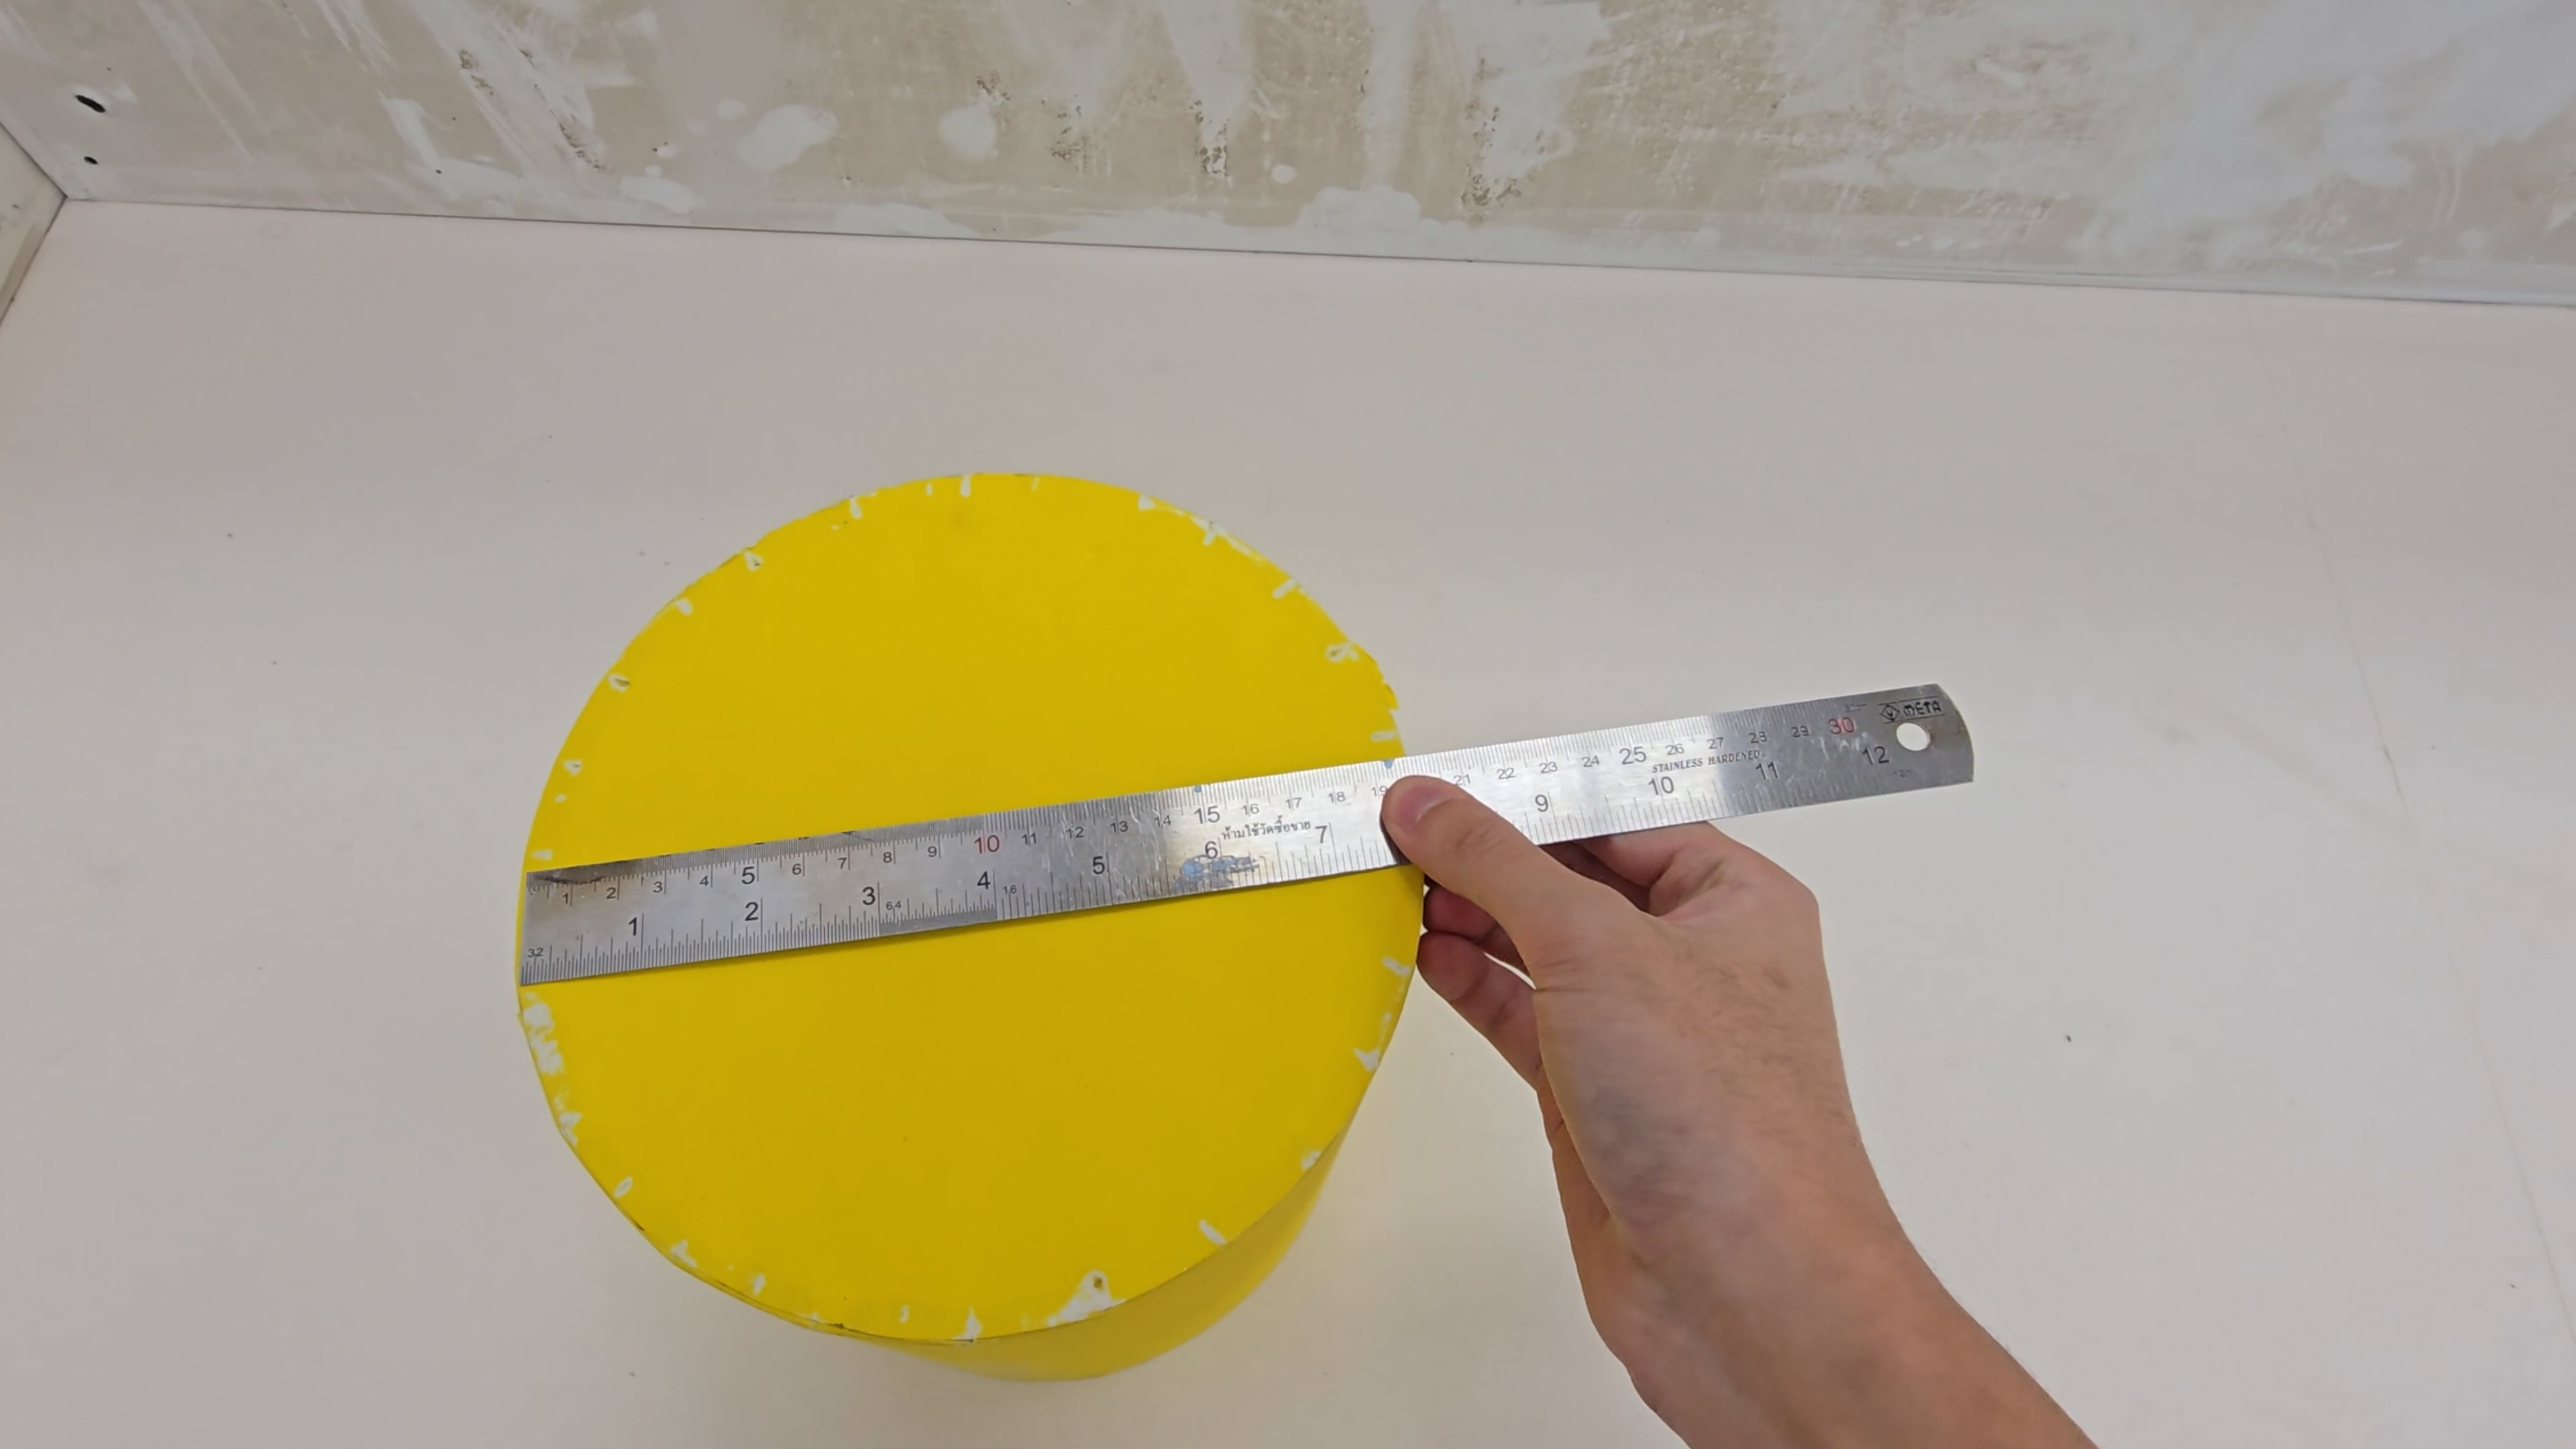
\includegraphics[width=1\linewidth]{assets/images/result-demo/AccurateCV 114-5-25-01:26-abr7500-0003.png}
    \caption{Accuracy of the measurements}
    \label{fig:detail-result}
\end{figure}

\paragraph*{}
The actual measurement is only off by around 5 cm. 

\begin{figure}[H]
    \centering
    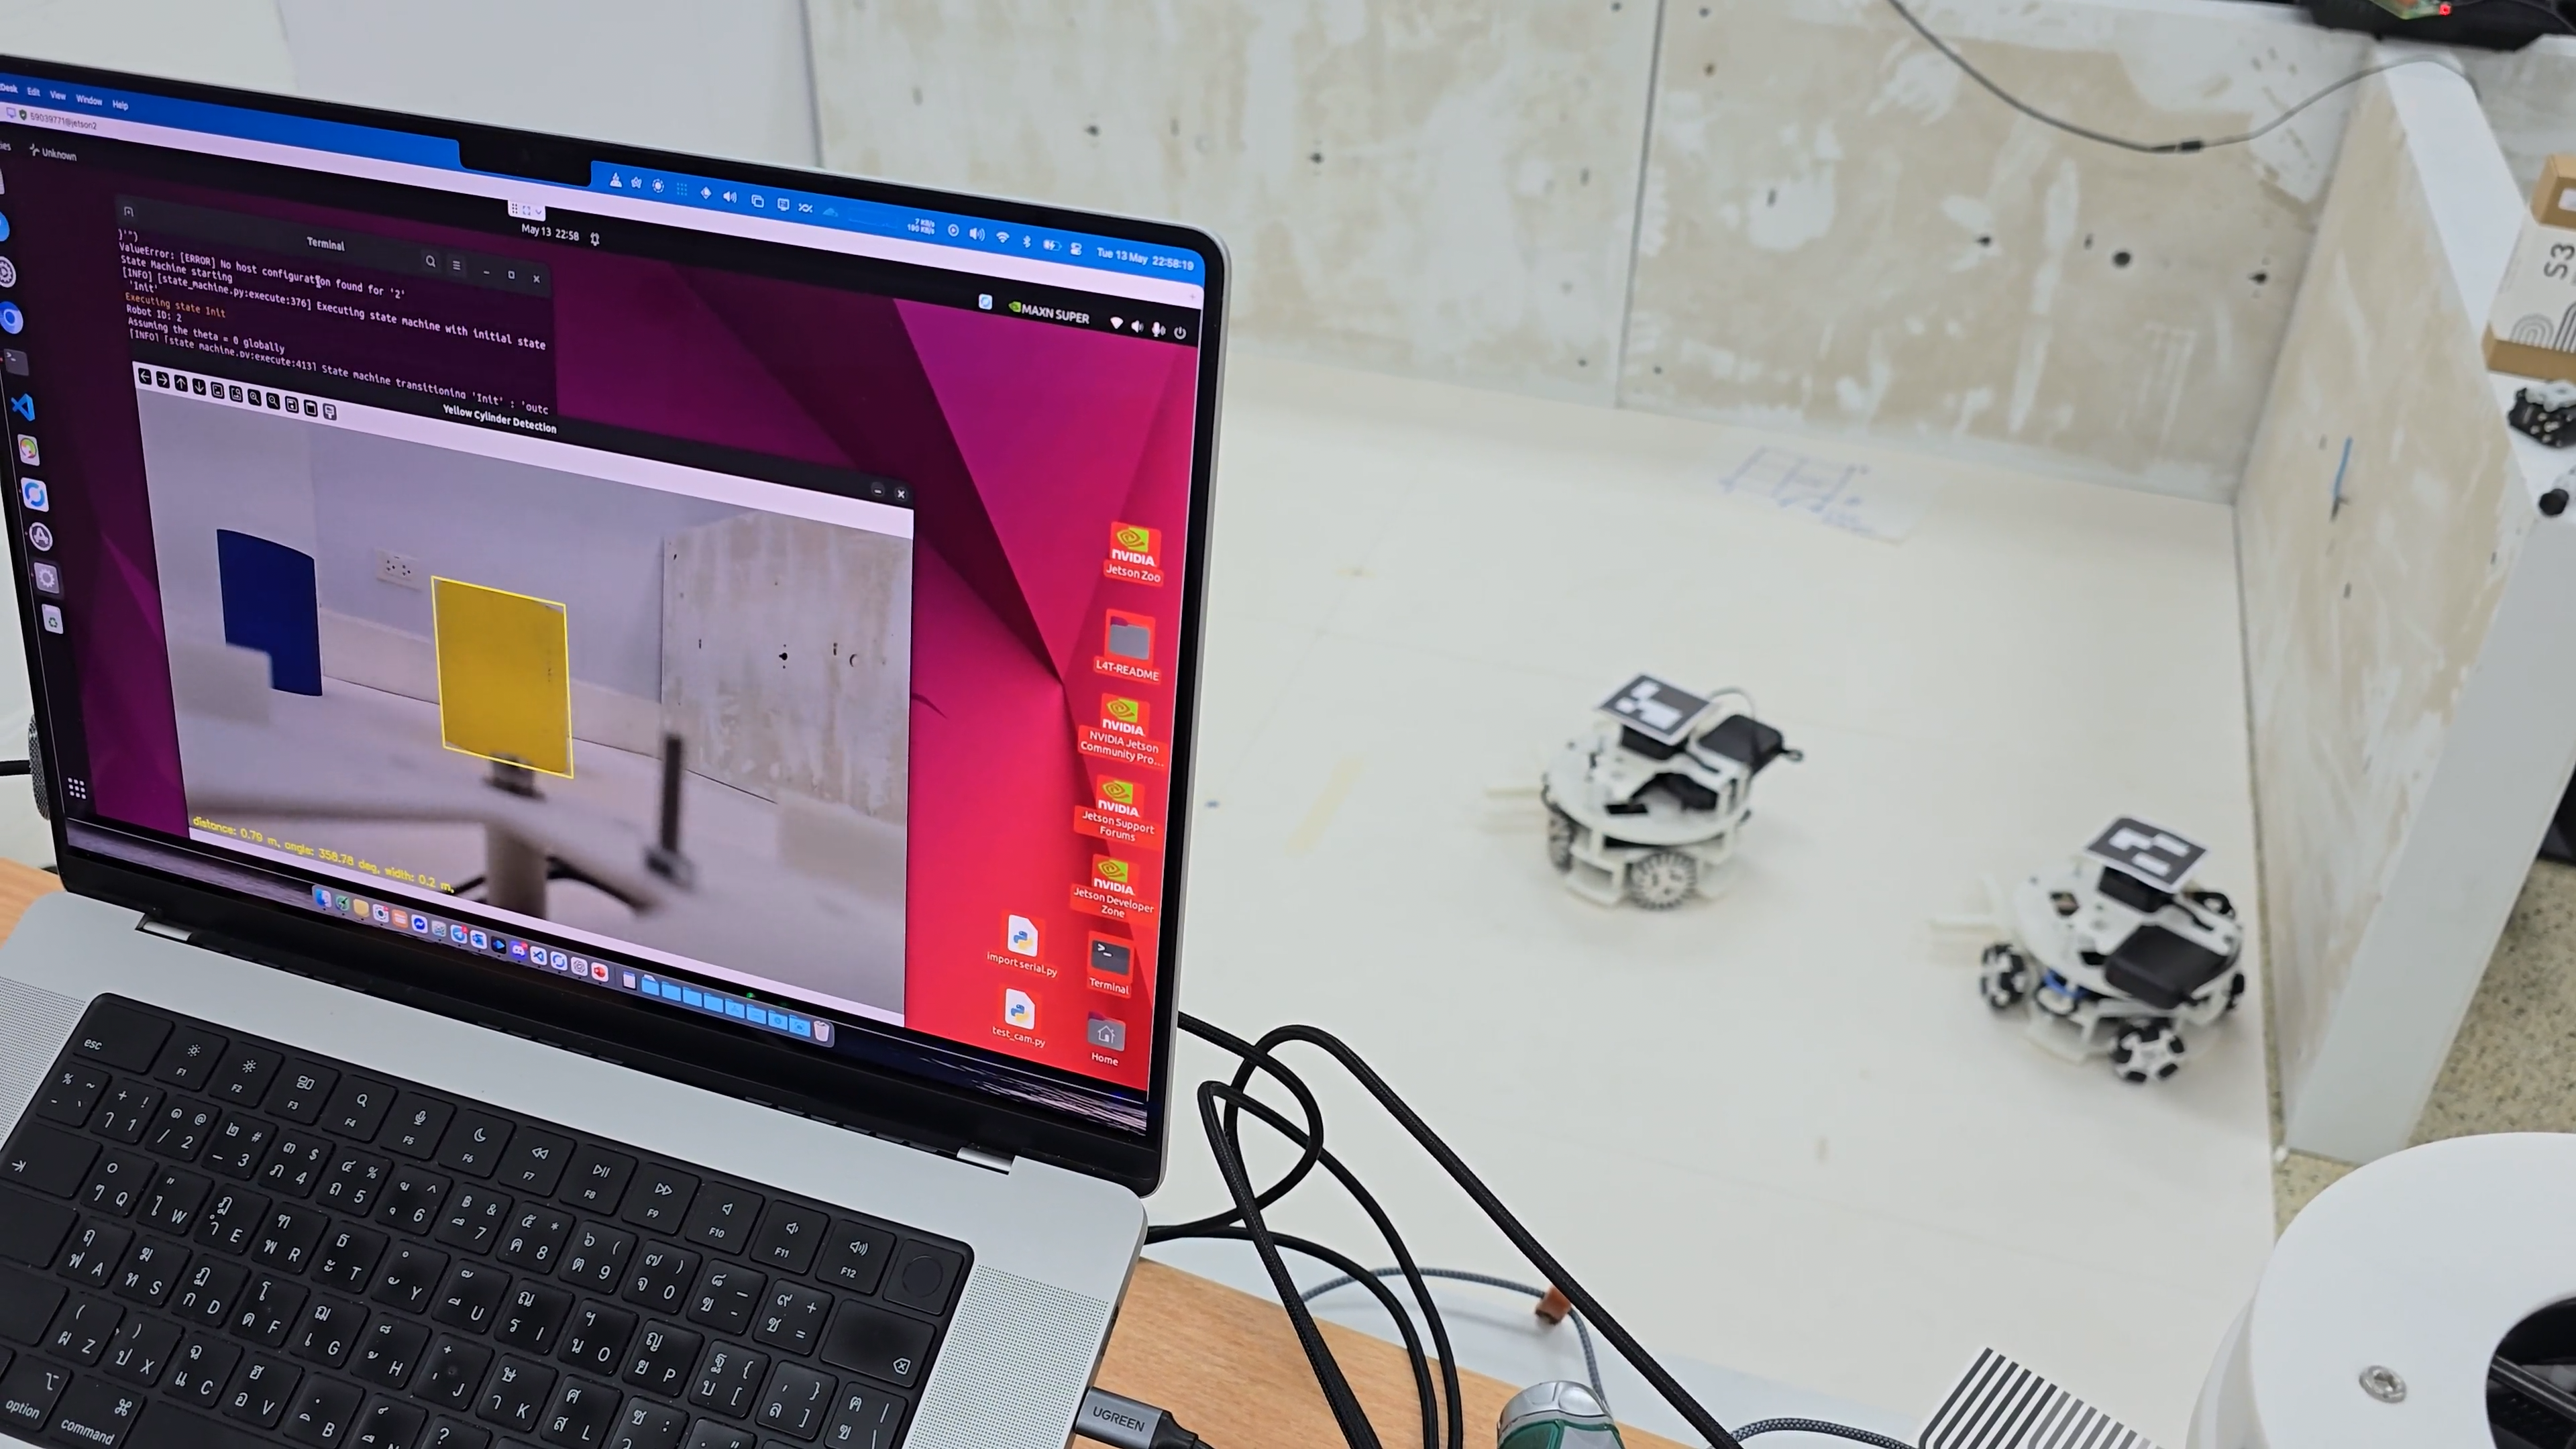
\includegraphics[width=1\linewidth]{assets/images/result-demo/ActivationCV 114-5-25-01:09-abr15000-0004.png}
    \caption{Robots navigating to object after detecting it}
    \label{fig:detail-result}
\end{figure}

\paragraph*{}
The robots after detecting the object then navigate towards it.